\documentclass[a4paper, 12pt,twoside]{book}

% set the paper size and the margins
\usepackage[top = 2cm, bottom = 2cm, left = 2cm, right = 4cm ]{geometry}
\usepackage[showboxes]{textpos}
\setlength{\TPHorizModule}{10mm}
\setlength{\TPVertModule}{\TPHorizModule}
\TPMargin{2mm}
% set the header and the footnote
\usepackage{fancyhdr}
% Supress the hyphenation
\hyphenation{thatshouldnot} 
% for table and equations
\usepackage{tablefootnote}
\usepackage{amsmath,amsfonts,amsthm}
\usepackage{hhline}
% make a wide hat for the least-squares regression line
 \usepackage{scalerel,stackengine}
\stackMath
\newcommand\reallywidehat[1]{%
\savestack{\tmpbox}{\stretchto{%
  \scaleto{%
    \scalerel*[\widthof{\ensuremath{#1}}]{\kern-.6pt\bigwedge\kern-.6pt}%
    {\rule[-\textheight/2]{1ex}{\textheight}}%WIDTH-LIMITED BIG WEDGE
  }{\textheight}% 
}{0.5ex}}%
\stackon[1pt]{#1}{\tmpbox}%
}
\usepackage[shortlabels]{enumitem}

% knitr packages
\usepackage[]{graphicx}
\usepackage[]{color}
%% maxwidth is the original width if it is less than linewidth
%% otherwise use linewidth (to make sure the graphics do not exceed the margin)
\makeatletter
\def\maxwidth{ %
  \ifdim\Gin@nat@width>\linewidth
    \linewidth
  \else
    \Gin@nat@width
  \fi
}
\makeatother

\definecolor{fgcolor}{rgb}{0.345, 0.345, 0.345}
\newcommand{\hlnum}[1]{\textcolor[rgb]{0.686,0.059,0.569}{#1}}%
\newcommand{\hlstr}[1]{\textcolor[rgb]{0.192,0.494,0.8}{#1}}%
\newcommand{\hlcom}[1]{\textcolor[rgb]{0.678,0.584,0.686}{\textit{#1}}}%
\newcommand{\hlopt}[1]{\textcolor[rgb]{0,0,0}{#1}}%
\newcommand{\hlstd}[1]{\textcolor[rgb]{0.345,0.345,0.345}{#1}}%
\newcommand{\hlkwa}[1]{\textcolor[rgb]{0.161,0.373,0.58}{\textbf{#1}}}%
\newcommand{\hlkwb}[1]{\textcolor[rgb]{0.69,0.353,0.396}{#1}}%
\newcommand{\hlkwc}[1]{\textcolor[rgb]{0.333,0.667,0.333}{#1}}%
\newcommand{\hlkwd}[1]{\textcolor[rgb]{0.737,0.353,0.396}{\textbf{#1}}}%
\let\hlipl\hlkwb
\usepackage{framed}
\makeatletter
\newenvironment{kframe}{%
 \def\at@end@of@kframe{}%
 \ifinner\ifhmode%
  \def\at@end@of@kframe{\end{minipage}}%
  \begin{minipage}{\columnwidth}%
 \fi\fi%
 \def\FrameCommand##1{\hskip\@totalleftmargin \hskip-\fboxsep
 \colorbox{shadecolor}{##1}\hskip-\fboxsep
     % There is no \\@totalrightmargin, so:
     \hskip-\linewidth \hskip-\@totalleftmargin \hskip\columnwidth}%
 \MakeFramed {\advance\hsize-\width
   \@totalleftmargin\z@ \linewidth\hsize
   \@setminipage}}%
 {\par\unskip\endMakeFramed%
 \at@end@of@kframe}
\makeatother


\definecolor{shadecolor}{rgb}{.97, .97, .97}
\definecolor{messagecolor}{rgb}{0, 0, 0}
\definecolor{warningcolor}{rgb}{1, 0, 1}
\definecolor{errorcolor}{rgb}{1, 0, 0}
\newenvironment{knitrout}{}{} % an empty environment to be redefined in TeX

\usepackage{alltt}


% packages will be used by the 'kable' package
\usepackage{booktabs}
\usepackage{longtable}
\usepackage{array}
\usepackage{multirow}
\usepackage[table]{xcolor}
\usepackage{wrapfig}
\usepackage{float}
\usepackage{colortbl} 
\usepackage{pdflscape}
\usepackage{tabu}
\usepackage{threeparttable}
\usepackage{threeparttablex}
\usepackage[normalem]{ulem}
\usepackage{makecell}
\usepackage{xcolor}
\IfFileExists{upquote.sty}{\usepackage{upquote}}{}

% define a color for highlight
\definecolor{asparagus}{rgb}{0.53, 0.66, 0.42}
\definecolor{babypink}{rgb}{0.96, 0.76, 0.76}
\definecolor{champagne}{rgb}{0.97, 0.91, 0.81}
\definecolor{forestgreen}{rgb}{0.13, 0.55, 0.13}
\definecolor{dollarbill}{rgb}{0.52, 0.73, 0.4}

\usepackage{tcolorbox}

\tcbset{width=0.9\textwidth,boxrule=0pt,colback=champagne,arc=0pt,
auto outer arc,left=0pt,right=0p}

\usepackage{hhline}

\usepackage{amsmath}

\setlength{\parindent}{0cm} 

\usepackage{siunitx}

%Chinese yen
\usepackage{stackengine}
\newcommand{\textyen}{\stackengine{-6pt}{=}{\large{\text{Y}}}{O}{c}{F}{T}{S}}

\setlength{\parindent}{0cm}

\begin{document}

%Deal with the headers of each chapter
\pagestyle{fancy}
\fancyhf{}
\renewcommand{\chaptermark}[1]{ \markboth{#1}{} }
\fancyhead[CE,CO]{\leftmark}
\fancyfoot[LE,RO]{\thepage}

\chapter{Confidence Intervals}
The purpose of sampling or experimentation is to make \textit{statistical inference} about the population. If the estimates of the parameters are given in the form of intervals, those intervals are called \textit{confidence intervals}.
\newpage

\section{Basics of confidence intervals}
\textbf{The following example throughout this section.}\vspace{0.3cm}

 To estimate the average height of all the high school students $\mathbf{\mu}$, we draw an SRS with $\overline{x} = 170$cm. What can we say about the parameter  $\mathbf{\mu}$?\vspace{0.3cm}
 
 You can say that $\mathbf{\mu} = 170$cm. In this case, the estimate only gives one value(170cm) for $\mathbf{\mu}$, this value is called \textbf{point estimate} and the statistic $\overline{x}$ is called a \textbf{point estimator}. \vspace{0.3cm}

$\overline{x}$ varies for different samples and it is hardly true that the real value of $\mathbf{\mu}$ is 170cm. In order to  take the chance variance of the the sampling distribution into account, an interval can be constructed to estimate the parameter . This interval is called the \textbf{confidence interval}.\vspace{0.3cm}

   \begin{itemize}
      \item \textbf{The idea of confidence interval}\vspace{0.3cm}
      
      The confidence interval is constructed by the following formula: 
      $$\textbf{statistic} \pm \textbf{margin of error}$$
      If the \textit{margin of error} is given, for each sample, we can construct a confidence interval by invoking the above formula. \vspace{0.3cm}
      
      If  $\mathbf{\overline{x}} = 170$cm, the confidence interval for $\mathbf{\mu}$ is\hspace{0.3cm} $170\text{cm} \pm \textbf{margin of error}$\\
            If  $\mathbf{\overline{x}} = 165$cm, the confidence interval for $\mathbf{\mu}$ is\hspace{0.3cm} $165\text{cm} \pm \textbf{margin of error}$\\
            $$\cdots\cdots\cdots\cdots\cdots\cdots\cdots\cdots$$
 Figure\ref{ConfidenceIntervals} gives the sampling distribution of $\overline{x}$ and the confidence intervals constructed on basis of different samples.
     \begin{figure}[H]
        \centering
        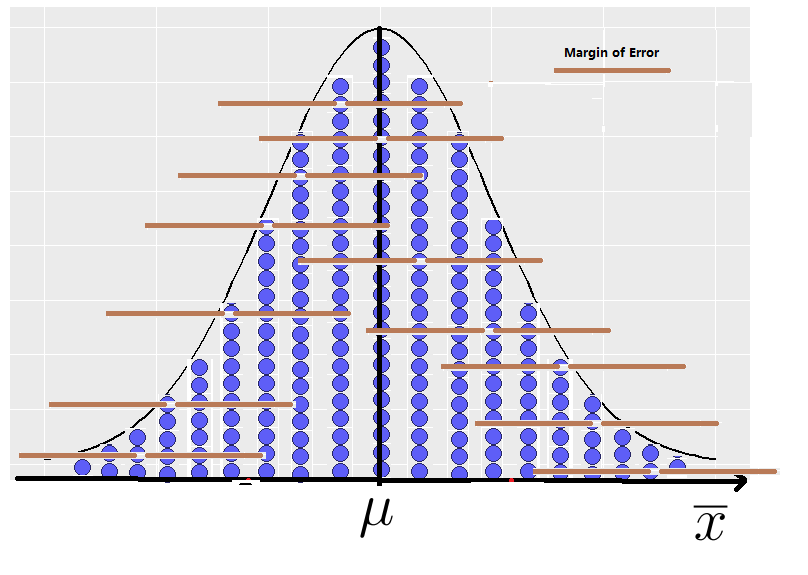
\includegraphics[scale=0.6]{ConfidenceIntervals}
        \vspace{-0.2cm}
        \caption{Confidence intervals}
        \label{ConfidenceIntervals}
     \end{figure}
  For samples with  $$\overline{x} \in [\mu - \textbf{ME},\; \mu + \textbf{ME}]\qquad(\textbf{ME} \text{ is short for} \textit{ margin of error})$$ 
   the confidence intervals can captures the $\mu$, others can not. A proper margin of error can be chosen such that \textbf{C}\% of all the possible confidence intervals can capture the parameter $\mu$. This ``\textbf{C}\%'' is called \textbf{confidence level}. 95\% is the most widely used confidence level. 
      \newpage
      \item \textbf{Interpreting confidence intervals and confidence levels}\vspace{0.6cm}
      

      \colorbox{babypink}{\parbox{\textwidth}{
            \textbf{Confidence interval} \vspace{0.3cm}
      
      Suppose we have constructed a confidence interval \textbf{[$a$, $b$]} with confidence level \textbf{C\%}.  It is interpreted as ``We are \textbf{C\%} confident that the interval from $a$ to $b$ captures the parameter(in context)'.'
      }}\vspace{0.3cm}
      
      For example, if [160, 180] is 95\% confidence interval for the average height of all high school students, it is interpreted as ``We are 95\% confident the interval from 160cm to 180cm can capture the average height of all high school studets.''\vspace{0.3cm}
      
      \textbf{Remarks:}
      \begin{itemize}[leftmargin = 0.5cm]
         \item The confident interval is constructed to estimate the \textit{parameter} not the \textit{statistic}. It's wrong to say ``We are \textbf{95\%} confident $\cdots\cdots$ can capture the average height of the sample.''
         \item It is wrong to say ``The probability the the interval [160, 180] can capture average height of all height school students is 95\%'', because the parameter $\mu$ is a fixed number not a random variable, and the interval [160, 180] is also fixed and the probability that [160, 180] can capture $\mu$ is either 0 or 1
         \item `` the parameter(in context)'' means you have to say it out clearly what is the parameter in the context. 
      \end{itemize}
      \vspace{0.6cm}
         
         \colorbox{babypink}{\parbox{\textwidth}{
         \textbf{Confidence level}\vspace{0.3cm}
         
         \textbf{C\%} confidence level is interpreted as ``If we draw many samples and construct confidence intervals by using the same formula, \textbf{C\%} of those intervals can capture the parameter(in context).''
         }}\vspace{0.6cm}
         
     \colorbox{champagne}{\parbox{\textwidth}{
     \textbf{Check Your Understanding}\vspace{0.3cm}
     
     How much does the fat content of Brand X hot dogs vary? To find out, researchers measured the fat content (in grams) of a random sample of 10 Brand X hot dogs. A 95\% confidence interval for the population standard deviation $\sigma$ is 2.84 to 7.55.
     \begin{enumerate}[(a)]
         \item Interpret the confidence interval.
         \item Interpret the confidence level.
         \item True or false: The interval from 2.84 to 7.55 has a 95\% chance of containing the actual population standard deviation s. Justify your answer.
     \end{enumerate}
     }}   

      
      
      
      
      
      
     \newpage 
      
      \item \textbf{The formula for confidence interval}\vspace{0.3cm}
      
      The confidence intervals for parameter $p$ and parameter $\mu$ are 
       $$\reallywidehat{p} \pm \textit{margin of error} \qquad \bar{x} \pm \textit{margin of error}$$
       $\reallywidehat{p}$ and $\bar{x}$ can be calculated from the sample directly. What about \textit{margin of error}? \vspace{0.6cm}     
       
       Refer to figure\ref{ConfidenceIntervals}. Suppose the conditions are met such that the sampling distribution of $\bar{x}$ is approximately normal: $\overline{x} \sim N(\mu, \sigma_{\bar{x}})$. Any sample with 
       $$\overline{x} \in [\mu - \textbf{ME},\; \mu + \textbf{ME}]\qquad(\textbf{ME} \text{ is short for} \textit{ margin of error})$$ 
       can result in a confidence interval captures the parameter $\mu$. If we want the \textit{confidence level} to be \textbf{C\%}, then
       $$\textbf{P}(\mu - \textbf{ME}\leq \overline{x} \leq \mu + \textbf{ME}) = \textbf{C\%} \implies \textbf{P}(\frac{-\textbf{ME}}{\sigma_{\overline{x}}}\leq \frac{\overline{x}-\mu}{\sigma_{\overline{x}}} \leq \frac{\textbf{ME}}{\sigma_{\overline{x}}}) = \textbf{C\%}$$
       $$\implies \textbf{P}(\frac{-\textbf{ME}}{\sigma_{\overline{x}}}\leq z_{\overline{x}} \leq \frac{\textbf{ME}}{\sigma_{\overline{x}}}) = \textbf{C\%}$$

       In the above equation, $\displaystyle{z_{\overline{x}} = \frac{\overline{x}-\mu}{\sigma_{\overline{x}}}}$, where $z_{\overline{x}}$ is the \textit{z-score} of $\overline{x}$. Since $\overline{x} \sim N(\mu, \sigma_{\bar{x}})$, $z_{\overline{x}}$ follows a \textit{standard normal distribution}, $z_{\overline{x}} \sim N(0, 1)$. 
     \begin{figure}[H]
         \centering
         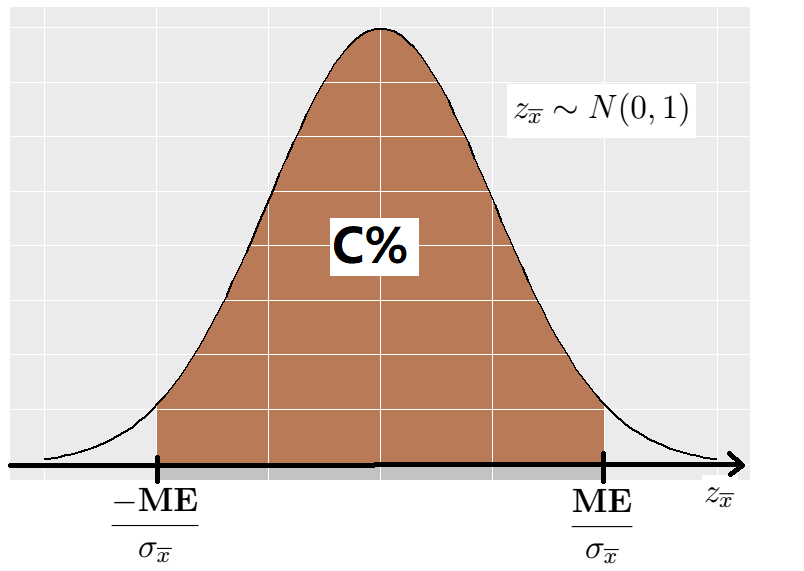
\includegraphics[scale=0.6]{ME}
         \caption{Calculate the \textbf{Margin of Error}}
         \label{ME}
     \end{figure}
           \begin{textblock}{4.8}(-3, -7)
      \textblockcolor{dollarbill}
      Why the \textbf{critical value} for the \textbf{95\%} confidence interval is 1.96?\vspace{0.3cm}
      
      What are the critical values for confidence interval with confidence levels \textbf{80\%, 90\%, 99\%}
      \end{textblock}
   Referring to figure\ref{ME}, if $\textbf{C\%} = 95\%$, then
      $$\frac{\textbf{ME}}{\sigma_{\overline{x}}}= 1.96 \implies \textbf{ME} = 1.96 \times \sigma_{\overline{x}} \qquad \sigma_{\overline{x}} = \frac{\sigma}{\sqrt{n}}$$ 
      The \textbf{95\% confidence interval} for $\mu$ is $\mathbf{\quad\bar{x} \pm 1.96\times \sigma_{\overline{x}}}$
      
      \colorbox{babypink}{\parbox{\textwidth}{
      The general formula for confidence interval is 
      $$\textbf{statistic} \pm (\textbf{critical value})\times (\textbf{standard devaition of the statistic})$$
  }}\vspace{0.6cm}
  
  
\item \textbf{Something more about the confidence interval}\vspace{0.3cm}

      And the \textit{margin of error} is given by
      
      \colorbox{babypink}{\parbox{\textwidth}{
                $$\textbf{Margin of Error} = (\textbf{critical value})\times (\textbf{standard devaition of the statistic})$$  
      }}\vspace{0.3cm}
      
       The standard deviation of $\reallywidehat{p}$ and $\overline{x}$ are given by
       $$\sigma_{\reallywidehat{p}} = \sqrt{\frac{p(1-p)}{n}} \qquad \sigma_{\overline{x}} = \frac{\sigma}{n}$$
       	where $p$ and $\sigma$ are parameters, and $n$ is the sample size.\vspace{0.3cm}
       	
       	\colorbox{babypink}{\parbox{\textwidth}{
       	\begin{itemize}[leftmargin = 0.5cm]
       	
       	    \item \textit{Confidence level C\%} does not change,  \textit{sample size n} increases. $\implies$\\
       	    
        \textit{Margin of Error} decreases.$\implies$ More precise estimate.\vspace{0.8cm}
        
          \item \textit{Confidence level C\%} increases,  \textit{sample size n} dose not change.$\implies$\\
       	    
        \textit{Margin of Error} increases.$\implies$ Less precise estimate.        
       	\end{itemize}
       	}}       	

If the sample size is kept the same, there is a trade-off between the confidence level and the precision of the estimate. More confident means low precision. This is intuitive just by considering the extreme case when the confidence level is 100\%, the \textit{margin of error} will be infinitely large.  \vspace{0.3cm}

If the confidence level is kept the same, and the sample size increase, which means the sample is more representative, and the estimation is more precise, thus a smaller margin of error.\vspace{0.3cm}

\colorbox{champagne}{\parbox{\textwidth}{
\textbf{Check the conditions!!!}\vspace{0.3cm}

  What conditions must be met for all the above formulas to hold?
}}

   \end{itemize}
\newpage

\section{One sample z-interval for population proportion}


The setting is: Draw an SRS of size $n$ and sample proportion $\reallywidehat{p}$, from a population of size $N$. Construct a C\% confidence interval for population proportion $p$. 
\vspace{0.6cm}
   
\begin{itemize}   
  \item \textbf{Check conditions}\vspace{0.3cm}
   
      In order to use apply the formulas in previous, we have to check conditions to make sure the sampling distribution of $\reallywidehat{p}$ can be approximated by normal distribution.\vspace{0.3cm}
      
   \begin{itemize}[leftmargin = 0.5cm]
       \item \textbf{Random:} The data should either come from a \textit{simple random sample} or an experiment with \textit{random assignments}. Otherwise, the formulas can not be used.\vspace{0.3cm}
       
       \begin{itemize}[leftmargin = 1cm]
           \item \textbf{10\% condition}. Make sure the sample size is no larger than 10\% of the population size. Because the individuals need to be independent to calculate the \textit{standard deviation of the statistics}
           $$\sigma_{\reallywidehat{p}} = \sqrt{\frac{p(1-p)}{n}}$$
         
       \end{itemize}
    \item \textbf{Large counts condition} \vspace{0.3cm}
    
       According to Chapter 6, if we want to approximate the sampling distribution of $\reallywidehat{p}$ with a normal distribution, we have to make sure the \textbf{10\% condition} is met, that is 
       $$np \geq 10 \qquad n(1-p) \geq 10$$ 
  However, we don't know the parameter $p$. We will use $\reallywidehat{p}$ to replace $p$. For \textit{10\% condition} we check 
      $$n\reallywidehat{p} \geq 10 \qquad n(1-\reallywidehat{p}) \geq 10$$
             
   \end{itemize}
   
   \begin{textblock}{3.6}(-3, -3)  
   \textblockcolor{dollarbill}
   Can you explain in detail why we have to check all those conditions ?
   \end{textblock}
   \vspace{0.6cm}

 \item\textbf{The formula}\vspace{0.3cm}
    $$\reallywidehat{p} \pm z^* \sqrt{\frac{p(1-p)}{n}}$$
    
    \begin{itemize}
        \item $\mathbf{z^*}$ is the critical value. Here we use $z^*$ means it is closely related to the \textit{z-score}. For 95\% confidence level, $z^* = 1.96$
        \item $\sigma_{\reallywidehat{p}}= \sqrt{\frac{p(1-p)}{n}}$. \hspace{0.3cm} Just like in the \textit{10\% condition},  $p$ is not known, and it is replaced by $\reallywidehat{p}$.
        
        
        $$\textbf{SE}_{\reallywidehat{p}} = \sqrt{\frac{\reallywidehat{p}(1-\reallywidehat{p})}{n}}$$
        
        $\textbf{SE}_{\reallywidehat{p}}$ is the \textbf{standard error of $\reallywidehat{p}$}. \vspace{0.3cm}
        
        When the standard deviation of a statistic is estimated from the statistic, the results is called the \textbf{standard error} of the statistic.
        
    \end{itemize}
    
    
\colorbox{babypink}{\parbox{\textwidth}{
\item \textbf{Put it all together}\vspace{0.3cm}

When you are asked to construct a confidence interval for population proportion $p$, you are supposed to do the following:

    \begin{itemize}
       \item \textbf{Identify appropriate confidence interval.}
       \item \textbf{Check conditions.}
       \item \textbf{Construct confidence interval by the formula}
       $$\reallywidehat{p} \pm z^* \sqrt{\frac{\reallywidehat{p}(1-\reallywidehat{p})}{n}}$$
       \item \textbf{Conclude and interpret.}
    \end{itemize}
    \vspace{0.6cm}
}}

    \newpage
    
\hspace{-1cm}    
\colorbox{champagne}{\parbox{\textwidth}{
\textbf{Example}\vspace{0.3cm}

Alcohol abuse has been described by college presidents as the number one problem on campus, and it is an important cause of death in young adults. How common is it? A survey of 10,904 randomly selected U.S. college students collected information on drinking behavior and alcohol-related problems. The researchers defined “frequent binge drinking” as having five or more drinks in a row three or more times in the past two weeks. According to this definition, 2486 students were classified as frequent binge drinkers. Construct and interpret a 99\% confidence interval for the proportion of binge drinkers among college students.\vspace{0.3cm}

\textbf{Solutions:}\vspace{0.3cm}

We should construct a one-sample z interval for the proportion $p$ of the frequent binge drinkers among college students if conditions are met.\vspace{0.6cm}

\textbf{Conditions:}
   \begin{itemize}
       \item \textbf{Random}. According to the problem, the 10,904 students were randomly selected.
       \begin{itemize}
          \item \textbf{10\% condition}, the sample size 10,904 is less than 10\% of all college students
       \end{itemize}
       \item \textbf{Large counts condition}
       $$n\reallywidehat{p}= 2, 486 \geq 10,  \qquad n()1-\reallywidehat{p} = 10,904 - 2,486 \geq 10$$
   \end{itemize}
   All the above conditions are met.\vspace{0.6cm}
   
   \textbf{Construct the confidence interval:}\vspace{0.3cm}
   
   The 99\% confidence interval for the proportion $p$ is given by 
   $$\reallywidehat{p} \pm z^* \sqrt{\frac{\reallywidehat{p}(1-\reallywidehat{p})}{n}}$$
   where $\reallywidehat{p} = \frac{2486}{10904} = 0.228$ and $z^* = 2.58$. \\
   The confidence interval for $p$ is 
   $$0.228 \pm 2.58\sqrt{\frac{0.228(1-0.228)}{10904}} = 0.228 \pm 0.010$$
   which is the interval (0.218, 0.238).\vspace{0.3cm}
   
   \textbf{Interpret:}\vspace{0.3cm}
   
   We are 99\% confident that the interval from 0.218 to 0.238 can capture the proportion of frequent binge drinkers among college students.
}}
\newpage
\colorbox{champagne}{\parbox{\textwidth}{
\textbf{Teens' Texting}\vspace{0.3cm}

 A Pew Internet and American Life Project survey found that 392 of 799 randomly selected teens reported texting with their friends every day. \vspace{0.3cm}
 
 \begin{enumerate}[(a)]
     \item Calculate and interpret a 95\% confidence  interval for the population proportion p that would report texting with their friends every day.
     \item Is it plausible that the true proportion of American teens who text with their friends every day is 0.45? Use your result from part (a) to support your answer.
 \end{enumerate} 
}}


\newpage

\item \textbf{Choosing proper sample size}\vspace{0.3cm}

In planning a study, we may want the margin of error restricted within certain range, that is 
$$z^* \sqrt{\frac{\reallywidehat{p}(1-\reallywidehat{p})}{n}} \leq \textbf{C}, \qquad \textbf{C} \textit{ is a given value.}$$
How to choose proper sample size $n$ such that the above inequality holds?\vspace{0.3cm}

Analyzing the inequality, we find that if we know the value of  $z^*$ and $\reallywidehat{p}$, we can solve $n$. $z^*$ is decided by the \textit{confidence level}. The only trouble is $\hat{p}$. There are two ways to find $\reallywidehat{p}$.
    \begin{itemize}
        \item Give $\reallywidehat{p}$ a reasonable guess according to pilot studies or past experiences.\vspace{0.3cm}
        
        \item Solve the inequality
        $$n \geq (\frac{z^*}{\textbf{C}})^2\;\reallywidehat{p}(1-\reallywidehat{p})$$
         $$\displaystyle{n \geq (\frac{z^*}{\textbf{C}})^2 \;0.5(1-0.5)
        \implies n \geq (\frac{z^*}{\textbf{C}})^2\; \reallywidehat{p}(1-\reallywidehat{p})\qquad \text{for any }  \reallywidehat{p}}$$\vspace{0.3cm}
        
         This means, if we let $\reallywidehat{p} = 0.5$ and solve $n$, then $n$ can make sure  $\textbf{ME} \leq \textbf{C}$. This estimation of $n$ is a \textbf{conservative estimation}.
    \end{itemize}
\end{itemize}
\vspace{0.6cm}

\colorbox{champagne}{\parbox{\textwidth}{
\textbf{Can you taste PTC?}\vspace{0.3cm}

 PTC is a substance that has a strong bitter taste for some people and is tasteless for others. The ability to taste PTC is inherited. About 75\% of Italians can taste PTC, for example. You want to estimate the proportion of Americans who have at least one Italian grandparent and who can taste PTC. 
 
 \begin{enumerate}[(a)]
     \item How large a sample must you test to estimate the proportion of PTC tasters within 0.04 with 90\% confidence? Answer this question using the 75\% estimate as the guessed value for $\reallywidehat{p}$.
     \item Answer the question in part (a) again, but this time use the conservative guess $\reallywidehat{p} = 0.5$. By how much do the two sample sizes differ?
 \end{enumerate}
}}
\newpage

\section{Two-sample z interval for $\mathbf{P_1- P_2}$}
The setting is: draw two SRS from two populations. The sample sizes are  $n_1$ and $n_2$, and sample proportion $\reallywidehat{p}_1$ and $\reallywidehat{p}_2$. Construct a C\% confidence interval for the difference between the two population proportions: $p_1-p_2$.\vspace{0.3cm}

 According the general formula for confidence interval 
 $$\textbf{statistic }\pm \textbf{critical valuse} \times \textbf{standard deviation of the statistic}, $$
 the confidence interval for $p_1-p_2$ is given by
 $$\reallywidehat{p}_1 - \reallywidehat{p}_2 \pm z^*\; \sigma_{\reallywidehat{p}_1 - \reallywidehat{p}_2 }$$
 
 \begin{itemize}
    \item \textbf{Check conditions}\vspace{0.3cm}
    
    In order to apply the above formulas, we have to make sure the sampling distribution of $\reallywidehat{p}_1- \reallywidehat{p}_2$ is approximately normal. We only have to make sure both the sampling distribution of $\reallywidehat{p}_1$ and $\reallywidehat{p}_2$ are normal, and they are independent. 
    
    \begin{textblock}{3}(15.5, -2)
    \textblockcolor{dollarbill}
    Why the sampling distributions of $\reallywidehat{p}_1$ and $\reallywidehat{p}_2$ are normal and independent?
    \end{textblock}
    
    \begin{itemize}
     \item \textbf{Independence}\vspace{0.3cm}
     
     Make sure the two set of data are independent.\vspace{0.3cm}
     
     \item\textbf{Random} \vspace{0.3cm}
     
     Both of the samples are random or both of the experiments are designed with \textit{random assignments}.
          \begin{itemize}
              \item \textbf{10\% condition}: Both of the two samples satisfy the 10\% condition.
          \end{itemize}
          
     \item \textbf{Large counts condition}\vspace{0.3cm}
      
      Both of the samples satisfy the large counts condition.
      
    \end{itemize}
    
            \begin{textblock}{4}(14, -1) 
   \textblockcolor{dollarbill}
    Describe the sampling distribution of $\reallywidehat{p}_1 - \reallywidehat{p}_2 $ if all the conditions are met.
   \end{textblock}
  
  \item \textbf{The formula} \vspace{0.3cm}
    
        $$\reallywidehat{p}_1 - \reallywidehat{p}_2 \pm z^*\; \sqrt{\frac{\reallywidehat{p}_1(1-\reallywidehat{p}_1)}{n_1} + \frac{\reallywidehat{p}_2(1-\reallywidehat{p}_2)}{n_2}}$$
        $$\textbf{SE}_{\reallywidehat{p}_1 - \reallywidehat{p}_2 }=\sqrt{\frac{\reallywidehat{p}_1(1-\reallywidehat{p}_1)}{n_1} + \frac{\reallywidehat{p}_2(1-\reallywidehat{p}_2)}{n_2}}$$
    
    \begin{textblock}{4}(14, -2)
    \textblockcolor{dollarbill}
    Can you prove the formula of $\textbf{SE}_{\reallywidehat{p}_1 - \reallywidehat{p}_2 }$
    \end{textblock}        
 \end{itemize}
 \vspace{1cm}
 
 \colorbox{babypink}{\parbox{\textwidth}{
  When constructing the confidence interval in \textbf{AP exam}, the general steps are the same as constructing one-sample z interval for $p$.
 }}
\newpage
\colorbox{champagne}{\parbox{\textwidth}{
\textbf{Teens and Adults on Social Networking Sites}\vspace{0.3cm}

As part of the Pew Internet and American Life Project, researchers conducted two surveys in 2012. The first survey asked a random sample of 799 U.S. teens about their use of social media and the Internet. A second survey posed similar questions to a random sample of 2253 U.S. adults. In these two studies, 80\% of teens and 69\% of adults used social-networking sites.\vspace{0.3cm}

Construct and interpret a 95\% confidence interval for the difference between the proportion of all U.S. teens and adults who use social-networking sites.
}}
\newpage
\section{One-sample z interval for population mean}

The setting is: draw an SRS of size $n$ from a population of size $N$ and standard deviation $\sigma$. The sample mean is $\overline{x}$. Construct a C\% confidence interval for population mean $\mu$.\vspace{0.3cm}

The formula for confidence interval is:
 $\displaystyle{\quad\overline{x} \pm z^*\;\sigma_{\overline{x}} \qquad \sigma_{\overline{x}} = \frac{\sigma}{\sqrt{n}}}$.
 
 \begin{itemize}
     \item \textbf{Check conditions:}\vspace{0.3cm}
     
     The above formula is built on basis that the sampling distribution of $\overline{x}$ is a normal distribution. We have to check related conditions to guarantee this.
     \begin{itemize}
        \item \textbf{Random}\vspace{0.3cm}
        
        The sample is random or the experiment is designed with \textit{random assignment}.
        \begin{itemize}
         \item \textbf{10\% condition:} the sample size is less than 10 percent of the population size.
        \end{itemize}
        
     \item \textbf{Normal/Large sample}\vspace{0.3cm}
     
     Check either of the following:
     \begin{itemize}
         \item The population has a normal distribution.
         \item The sample size $n \geq 30$.
         \item The distribution of the sample data is  roughly symmetric and no obvious outliers, and thus it is reasonable to assume the population distribution is approximately normal.\vspace{0.3cm}
         
            \colorbox{babypink}{\parbox{0.8\textwidth}{
  \textbf{Those three conditions are check in the order as listed until one of them is satisfied.}
   }}
     \end{itemize}    
     \end{itemize}
      \vspace{0.6cm}
      
             
    \item \textbf{The formula}    
    $$\overline{x} \pm z^*\;\frac{\sigma}{\sqrt{n}}$$
    Here, we know $\sigma$. We don't use $\textbf{SE}_{\overline{x}}$, for .
 \end{itemize}
 \begin{textblock}{4.5}(14, -2) 
   \textblockcolor{dollarbill}
    Describe the sampling distribution of $\overline{x}$ if all the conditions are met.
   \end{textblock}
 \newpage
 \section{Two-sample z interval for $\mathbf{\mu_1 - \mu_2}$}
 
 The setting is: draw two samples of sizes $n_1$ and $n_2$, sample means $\overline{x}_1$ and $\overline{x}_2$, from two populations with population standard deviations $\sigma_1$ and $\sigma_2$. Construct a C\% confidence interval for $\mu_1-\mu_2$\vspace{0.3cm}
 
 The formula for this confidence interval is:
 $$\overline{x}_1 - \overline{x}_2 \pm z^*\; \sigma_{\overline{x}_1 - \overline{x}_2}$$
 
 \begin{itemize}
     \item \textbf{Check conditions}\vspace{0.3cm}
     
     In order to apply the formula given above, we have to make sure the sampling distribution of $\overline{x}_1 - \overline{x}_2 $ is approximately normal by checking certain conditions.
     \begin{itemize}
        \item \textbf{Independence}\vspace{0.3cm}
        
        The two simple random sample are independent
        
        \item \textbf{Random}\vspace{0.3cm}
        
        The samples are simple random samples or the experiments are designed by random assignments
        
        \begin{itemize}
           \item \textbf{10\% condition.} Both the two samples satisfy the \textit{10\% condition}.
        \end{itemize}
        
        \item \textbf{Normal/Large sample}\vspace{0.3cm}
        
        Check either of the following for both of the samples.
        \begin{itemize}
                     \item The population has a normal distribution.
         \item The sample size $n \geq 30$.
           \item The distribution of the sample data is  roughly symmetric and no obvious outliers, and thus it is reasonable to assume the population distribution is
        \end{itemize}
        
     \end{itemize}
     
        \begin{textblock}{4.5}(-3.2, -2.5) 
   \textblockcolor{dollarbill}
    Describe the sampling distribution of $\overline{x}_1 - \overline{x}_2$ if all the conditions are met.
   \end{textblock}
   
 \item \textbf{The formula}  \vspace{0.3cm}  
 
     $$\overline{x}_1 - \overline{x}_2 \pm z^*\; \sqrt{\frac{\sigma_1^2}{n_1} + \frac{\sigma_2^2}{n_2}}$$

 \end{itemize}
 
   \begin{textblock}{4.8}(-3.2, -2.5) 
   \textblockcolor{dollarbill}
   Can you deduce the formulas?\vspace{0.3cm}
   
   Why don't we use $\textbf{SE}_{\overline{x}_1 - \overline{x}_2 }$?
   \end{textblock}
   \newpage
   \colorbox{champagne}{\parbox{\textwidth}{
   \textbf{Who is taller?}\vspace{0.3cm}
   
    The heights of young men follow a Normal distribution with  standard deviation 2.8 inches. The heights of young women follow a Normal distribution with standard deviation 2.5 inches. Suppose we select independent SRSs of 16 young men and 9 young women. The sample mean heights  of young men is:  $\overline{x}_M = 69.3$ inches. The sample young women heights is: $\overline{x}_W = 64.5$ inches\vspace{0.3cm}
    
    Construct a 90\% confidence interval for the difference of the mean heights be young men and young women.
   }}
   
   \newpage
   
   \section{t intervals for population mean}
   In previous section we learned how to construct confidence intervals for population means with population standard deviation known. However, most of the time if we don't know the population we don't know the population standard deviation. People may say, we can replace the population standard deviation with the sample standard deviation and apply the above formulas. The situation is different here. If population standard deviation is replaced by the sample standard deviation, the sampling distribution is the \textit{t-distribution}.\vspace{0.3cm}
   
   Suppose the C\% confidence interval for population mean 
   $\mu$ is $$\overline{x} \pm \textbf{ME}$$ 
   where \textbf{ME} is short for the \textit{margin of error}. Suppose the sampling distribution of $\overline{x}$ is normal. Referring to section 1, we have the following:
   
   \begin{equation*}
   \begin{split}
   \textbf{P}(\mu - \textbf{ME} \leq \overline{x} \leq \mu + \textbf{ME}) &= \textbf{C\% }\\   
\textbf{P}(\frac{-\textbf{ME}}{s_{x}/\sqrt{n}}\leq \frac{\overline{x}-\mu}{s_{x}/\sqrt{n}} \leq \frac{\textbf{ME}}{s_{x}/\sqrt{n}})& = \textbf{C\%} \\
   \textbf{P}(\frac{-\textbf{ME}}{\textbf{SE}_{\overline{x}}}\leq \frac{\overline{x}-\mu}{\textbf{SE}_{\overline{x}}} \leq \frac{\textbf{ME}}{\textbf{SE}_{\overline{x}}}) &= \textbf{C\%} \\
    \textbf{P}(\frac{-\textbf{ME}}{\textbf{SE}_{\overline{x}}}\leq t_{\overline{x}} \leq \frac{\textbf{ME}}{\textbf{SE}_{\overline{x}}}) &= \textbf{C\%} \\            
    \end{split}          
 \end{equation*}
 In the above equation, $t_{\overline{x}}$ follows the \textit{t-distribution} with \textit{degree of freedom} $dg = n-1$, where $n$ is the sample size.
    \begin{figure}[H]
       \centering
       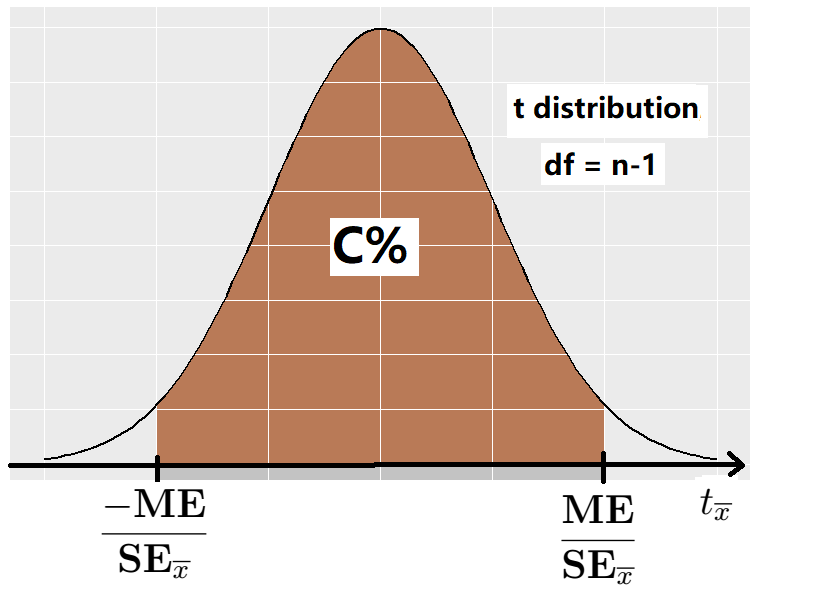
\includegraphics[scale=0.6]{tInterval}
       \caption{t interval}
       \label{tInterval}
    \end{figure}
    
    \begin{textblock}{4.8}(-3, -7)
    \textblockcolor{dollarbill}
    Find $t^*$ for the following cases
    \begin{itemize}[leftmargin = 0.3cm]
      \item $n=5, \quad \textbf{C\%} = 95\%$
      \item $n=10, \quad \textbf{C\%} = 95\%$
      \item $n=20, \quad \textbf{C\%} = 95\%$
    \end{itemize}
    \end{textblock}
    As shown in figure\ref{tInterval}, suppose $\displaystyle{t^* = \frac{\textbf{ME}}{\textbf{SE}_{\overline{x}}}}$, then $\textbf{ME} = t^*\times \textbf{SE}_{\bar{x}}$. The t-interval is 
    $$\bar{x}\pm t^*\times \textbf{SE}_{\bar{x}}$$
    $t^*$ is the \textbf{critical value}, and the formula is consistent with
    $$\textbf{statistic} \pm (\textbf{critical value})\times (\textbf{standard error of the statistic})$$
    
    \newpage
    
  \begin{itemize}
      \item \textbf{One-sample t interval for population mean}\vspace{0.3cm}
      
      The setting of this type of interval is exactly the same as \textit{one-sample z interval for population mean}, except that we don't know the population standard deviation $\sigma$.\vspace{0.3cm}
      
      The conditions to check are exact the same as the conditions to check in \textit{one-sample z interval for population mean}.\vspace{0.3cm}
      
      \textbf{The formula:}
      
          $$\bar{x}\pm t^* \; \frac{s_X}{\sqrt{n}}$$
     The degree of freedom of $t^*$ is $n-1$
  \item \textbf{Two-sample t interval for $\mu_1-\mu_2$}        \vspace{0.3cm}
  
  What is true for \textit{one-sample t interval} is also true here.\vspace{0.3cm}\vspace{0.3cm}
  
  \textbf{The formula:}\vspace{0.3cm}
  
   $$\bar{x}_1-\bar{x}_2\pm t^* \; \sqrt{\frac{s_1^2}{n_1} + \frac{s_2^2}{n_2}}$$
   $$\textbf{SE}_{\bar{x}_1-\bar{x}_2} = \sqrt{\frac{s_1^2}{n_1} + \frac{s_2^2}{n_2}}$$
   
    \begin{textblock}{4.8}(13.5, -5)
 \textblockcolor{dollarbill}
  Can you deduce the formula of $\textbf{SE}_{\bar{x}_1}$?
  
   The $t$ statistic of $\bar{x}$ is given by $$t = \frac{\bar{x}-\mu}{s_x/\sqrt{n}}$$
   Can you find the formula for the $t$ statistic of $\bar{x}_1 - \bar{x}_2$
 \end{textblock}

    
 The degree of freedom are given by one of the two methods.
     \begin{itemize}
        \item $df=\text{min}(n_1-1, n_2-1)$, this is a \textbf{conservative} way.
        \item $\displaystyle{df = \frac{(\frac{s_1^2}{n_1}+\frac{s_2^2}{n_2})^2}
        {\frac{1}{n_1-1}(\frac{s_1^2}{n_1})^2 + \frac{1}{n_2-1}(\frac{s_2^2}{n_2})^2}}$
        This will be given by the calculator.
     \end{itemize}
\textbf{ In practice, we just report the $df$ given by the calculator.}

 \vspace{0.6cm}
 
 \colorbox{babypink}{\parbox{\textwidth}{
 \textbf{Remark:}
 
 \begin{itemize}
     \item Confidence intervals are for parameters.
     \item There is no t intervals for populations proportions.
     \item For population means, t intervals are more frequently used than z intervals 
     \item The steps of constructing confidence t intervals are the same as of z intervals.  \textbf{The only difference is you have to report the \textit{degree of freedom} of $t^*$ when constructing t intervals.}   
 \end{itemize}
 }}
 
  \newpage
  
 \item \textbf{Choosing proper sample size}\vspace{0.3cm}
 
 Sometimes we have to choose proper sample size such that the margin of error is less than a specified value, say C.
 $$\textit{Margin of error}\; = t^*\;\frac{s_x}{\sqrt{n}}\leq \textbf{C}$$
 The problem of solving $n$ is $t^*$ depends on \textit{the degree of freedom}, which is $n-1$, and $s_x$ is related to the sample size $n$ as well. We do the following two things to simplify:
 \begin{itemize}
     \item Replace $t^*$ by $z^*$ which is totally decided by the confidence level C\%.
     \item Replace $s_x$ by some value, say $\sigma$, from a pilot study or past experience, or a reasonable guess.
 \end{itemize}
 Thus the inequality becomes \hspace{0.3cm}
     $\displaystyle{ z^*\;\frac{\sigma}{\sqrt{n}}\leq \textbf{C}}$. \hspace{0.3cm} Easy to solve for $n$.
   \end{itemize} \vspace{0.3cm}

 \colorbox{champagne}{\parbox{\textwidth}{
 \textbf{How many monkeys}\vspace{0.3cm}
 
 Researchers would like to estimate the mean cholesterol level m of a particular  variety of monkey that is often used in laboratory experiments. They would like their estimate to be within 1 milligram per deciliter (mg/dl) of the true value of m at a 95\% confidence level. A previous study involving this variety of monkey suggests that the standard deviation of cholesterol level is about 5 mg/dl.\vspace{0.3cm}
 
 Obtaining monkeys for research is time-consuming, expensive, and controversial. What is the minimum number of monkeys the researchers will need to get a satisfactory estimate?
 }}
 \newpage
 
  \colorbox{champagne}{\parbox{\textwidth}{
 \textbf{Self-healing }\vspace{0.3cm}
 
 Biologists studying the healing of skin wounds measured the rate at which new cells closed a cut made in the skin of an anesthetized newt. Here are data from a random sample of 18 newts, measured in micrometers (millionths of a meter) per hour:
 \begin{table}[H]
 \centering
    \begin{tabular}{c}
     \hline
     29\hspace{0.2cm} 27\hspace{0.2cm} 34\hspace{0.2cm} 40\hspace{0.2cm} 22 \hspace{0.2cm}28 \hspace{0.2cm}14 \hspace{0.2cm}35\hspace{0.2cm} 26 \hspace{0.2cm}35 \hspace{0.2cm}12 \hspace{0.2cm}30 \hspace{0.2cm}23\hspace{0.2cm} 18 \hspace{0.2cm}11 \hspace{0.2cm}22 \hspace{0.2cm}23 \hspace{0.2cm}33\\
     \hline
    \end{tabular}
    \vspace{0.3cm}
     \end{table}
     
    Calculate and interpret a 95\% confidence interval for the mean healing rate.
 }}
 \newpage
 \colorbox{champagne}{\parbox{\textwidth}{
 \textbf{Tropical Flowers}\vspace{0.3cm}
 
  Different varieties of the tropical flower \textit{Heliconia} are fertilized by different species of hummingbirds. Researchers believe that over time, the lengths of the flowers and the forms of the hummingbirds’ beaks have evolved to match each other. Here are data on the lengths in millimeters for random samples of two color varieties of the same species of flower on the island of Dominica:
  \begin{table}[H]
  \hspace{-0.5cm}
  \small{
   \begin{tabular}{ccccc ccccc cc}
   \hline
   \multicolumn{12}{c}{\textbf{H.\textit{ caribaea} red}}\\
   41.90&42.01&41.93&43.09&41.17&41.69&39.78&40.57&
   39.63 & 42.18 & 40.66 & 37.87 \\
   39.16 & 37.40 & 38.20&  38.07 & 38.10 & 37.97 & 38.79 &       38.23 & 38.87 & 37.78 & 38.01&\\
   \hline
   \end{tabular}
   }
  \end{table} 
    \begin{table}[H]
  \hspace{-0.5cm}
  \small{
   \begin{tabular}{ccccc ccccc cc}
   \hline
   \multicolumn{12}{c}{\textbf{H.\textit{ caribaea} yellow}}\\
36.78 &37.02 &36.52 &36.11 &36.03& 35.45& 38.13 &37.10 &35.17 &36.82 &36.66 &35.68 \\
36.03 &34.57 &34.63 \\
   \hline
   \end{tabular}
   }
  \end{table}
  \begin{enumerate}[(a)]
      \item Draw two boxplots to compare the distribution of the two samples.
      \item Construct and interpret a 95\% confidence interval for the difference in the mean lengths of these two varieties of flowers.
      \item Does the interval support the researchers’ belief that the two flower varieties have different average lengths? Explain.
  \end{enumerate} 
 }}
    
\end{document}